
% this file is called up by thesis.tex
% content in this file will be fed into the main document

% ----------------------- introduction file header -----------------------
%\chapter{Search for the FCNC decay \pmb{$t\rightarrow c + Z$}}
\chapter{Search for the FCNC decay of top-quark in \Pqc-quark and Z boson}
\label{chapter:analysis}

% the code below specifies where the figures are stored
\graphicspath{Chapters/CH6/figures}

% ----------------------------------------------------------------------
% ----------------------- introduction content -------------------------
% ----------------------------------------------------------------------


\section{Event selections and reconstruction}
\label{sec:selection}

\subsection {Signal Region definition}
\label{sec:sel:sr3}
\clearpage
\section{Background estimation}
\label{sec:background}

\subsection {Control Regions definition}
\label{sec:bkg:sel}
In the following, the event selection in the CRs is described.\\
\Cref{tab:bkg:crs} summarises the selection cuts in the various CRs.
\paragraph{\ttbar CR selections}
The \ttbar CR is defined by requiring that there is at least one pair
of opposite-sign but different-flavour leptons in the
event. Obviously, no cut on the invariant mass of the opposite-sign
leptons is applied. Concerning the jet multiplicity, there should be
at least one jet in the event, of which exactly one should be
\Pqb-tagged.

\paragraph{\ttZ CR selections}
\label{sec:bkg:ttz}
The \ttZ CR is defined by requiring the presence of at least four jets
and of exactly two \Pqb-tagged jets. Also the cut on the transverse
mass of the \PW boson is softened to \SI{30}{\GeV}. To be orthogonal 
with SR3, also a veto on the presence of a c-jet is required. 

\paragraph{Side-band CR1 selections}
\label{sec:bkg:sbcr1tzu}
The mass side-band CR1 is defined by requiring the presence of at least two jets
and of exactly one \Pqb-tagged jet.
The mass of the FCNC top-quark candidate, \mtopfcnc,
must be outside $2\sigma^{FCNC}$ from \mtopvalue, the mass of the
SM top-quark candidate, \mtopsm, must be also outside $2\sigma^{SM}$
from \mtopvalue.  In addition, a veto on the presence of a c-jet is required. 

\paragraph{Side-band CR2 selections}
\label{sec:bkg:sbcr2}
The mass side-band CR2 is defined by requiring the presence of exactly one or two jets
and of exactly one \Pqb-tagged jet.   The transverse mass is calculated using the momentum of the lepton associated with the $W$ boson, $\MET$ and azimuthal angle,$\phi$, between them: 
$\mT(\ell_{\PW},\Pgn) = \sqrt{2\pT^{\ell}\MET \left(1-\cos\Delta\phi\right)}$.
Events are required to have $\mT(\ell_{\PW},\Pgn) > \SI{40}{\GeV}$.\\
The mass of the SM top-quark candidate, \mtopsm, must be also outside $2\sigma^{SM}$
from \mtopvalue.\\
Event yields in the CRs are shown in \Cref{tab:bkg:yields:tzc}. 
As it can be noticed, the signal contribution in the various CRs is small.
\begin{table}[htbp]
	\small
	\caption{Event yields in the CRs for the \tZc coupling extraction. \TabErrStatSys} 
	\label{tab:bkg:yields:tzc}
	\centering
	% NB: add to main document: 
% \usepackage{siunitx} 
% \sisetup{separate-uncertainty,table-format=6.3(6)}  % hint: modify table-format to best fit your tables
\begin{tabular}{|l|S|S|S|S|}
\toprule  
 & {Side-band CR1} & {Side-band CR2} & {\ttZ CR} & {\ttbar CR}\\
\midrule 
  \ttZ+\tWZ   & 88 \pm 12 & 9.1 \pm 2.1 & 164 \pm 22 & 14.8 \pm 1.9 \\ 
  \ttW   & 4.3 \pm 0.7 & 2.5 \pm 0.5 & 2.3 \pm 0.5 & 27 \pm 4 \\ 
  \ttH   & 2.3 \pm 0.4 & 0.36 \pm 0.07 & 5.4 \pm 0.9 & 13.8 \pm 2.1 \\ 
  \VVLF   & 25 \pm 15 & 18 \pm 7 & 0.20 \pm 0.22 & 0.40 \pm 0.21 \\ 
  \VVHF   & 130 \pm 80 & 69 \pm 28 & 13 \pm 11 & 2.3 \pm 1.4 \\ 
  \tZq   & 20 \pm 4 & 9.9 \pm 1.7 & 14.6 \pm 2.9 & 0.90 \pm 0.15 \\ 
  \ttbar+Wt   & 10 \pm 4 & 9.1 \pm 2.7 & 3.0 \pm 1.2 & 102 \pm 24 \\ 
  Other fakes   & 3 \pm 5 & 10 \pm 11 & 0.00 \pm 0.06 & 0.12 \pm 0.14 \\ 
  Other   & 2.2 \pm 1.6 & 0.8 \pm 2.6 & 1.1 \pm 0.5 & 2.9 \pm 1.5 \\ 
\midrule 
  Total background  & 280 \pm 80 & 130 \pm 32 & 203 \pm 27 & 164 \pm 25 \\ 
\midrule 
  Data   & 331 & 169 & 197 & 156 \\ 
\midrule 
  Data / Bkg.   & 1.18 \pm 0.35 & 1.30 \pm 0.34 & 0.97 \pm 0.14 & 0.95 \pm 0.16 \\ 
\bottomrule 
\end{tabular} 

\end{table} 

\clearpage
\global\pdfpageattr\expandafter{\the\pdfpageattr/Rotate 90}
\begin{sidewaystable}[!htbp]
	\caption{
		Overview of the requirements applied for selecting events in the control regions.
	}%
	\label{tab:bkg:crs}
	\centering
	\footnotesize
	\begin{tabular}{c|c|c|c}
		\toprule
		\multicolumn{4}{c}{Common selections} \\
		\midrule
		\multicolumn{4}{c}{Exactly 3 leptons with $|\eta| < 2.5$ and $\pT(\ell_1)> \SI{27}{\GeV}$, $\pT(\ell_2)> \SI{15}{\GeV}$, $\pT(\ell_3)> \SI{15}{\GeV}$} \\
		\midrule
		\ttbar CR & \ttZ CR & Side-band CR1 & Side-band CR2 \\
		\midrule
		$\ge$ 1 \OS pair, no \OSSF  & $\ge$ 1 \OSSF pair & $\ge$ 1 \OSSF pair & $\ge$ 1 \OSSF pair \\
		& with $|\mll - \SI{91.2}{\GeV}| < \SI{15}{\GeV}$ & with $|\mll - \SI{91.2}{\GeV}| < \SI{15}{\GeV}$ & with $|\mll - \SI{91.2}{\GeV}| < \SI{15}{\GeV}$ \\
		-- & $\mT(\ell_{\PW},\Pgn) > \SI{30}{\GeV}$ & $\mT(\ell_{\PW},\Pgn) > \SI{40}{\GeV}$ & $\mT(\ell_{\PW},\Pgn) > \SI{40}{\GeV}$ \\
		$\ge$ 1 jet with $|\eta| < $ 2.5  & $\ge$ 4 jet with $|\eta| < $ 2.5 & $\ge$ 2 jet with $|\eta| < $ 2.5  & = 1 jet with $|\eta| < $ 2.5 \\
		= 1 \Pqb-jet  & = 2 \Pqb-jet  &  = 1 \Pqb-jet & = 1 \Pqb-jet \\
		-- & -- & = 0 c-jet & --\\ 
		-- & -- &  $|\mtopfcnc - \mtopvalue| > 2\sigma^{FCNC}$ & -- \\
		-- & -- & $|\mtopsm - \mtopvalue| > 2\sigma^{SM}$ & $|\mtopsm - \mtopvalue| > 2\sigma^{SM}$ \\
		\bottomrule
	\end{tabular}
\end{sidewaystable} 
\clearpage
\FloatBarrier
\subsubsection{\ttbar CR}
%
\global\pdfpageattr\expandafter{\the\pdfpageattr/Rotate 0} -------------------------------------------------------------------------------
\Cref{fig:sel:cr:ttbar:leps,fig:sel:cr:ttbar:jets} show the distributions 
of kinematic variables for events selected in the \ttbar CR region.

\begin{figure}[!htbp]
	\centering
	\begin{tabular}{cc}
		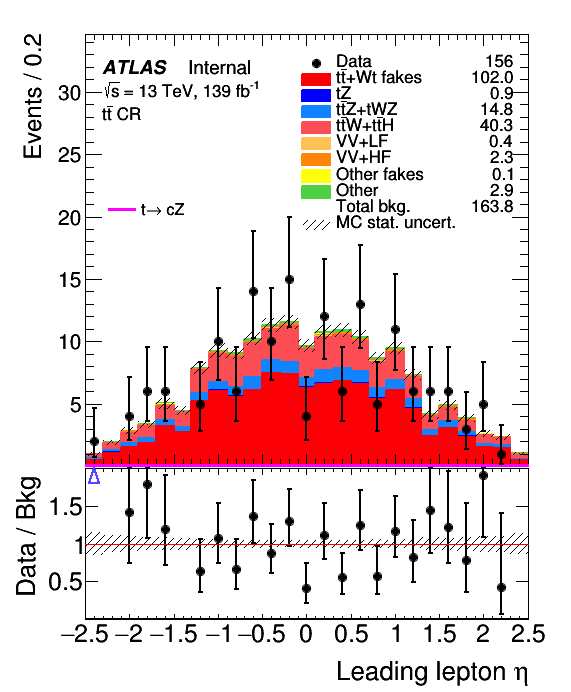
\includegraphics[width=.32\textwidth]{Chapters/CH6/figures/TTCR/lep1_eta} &
		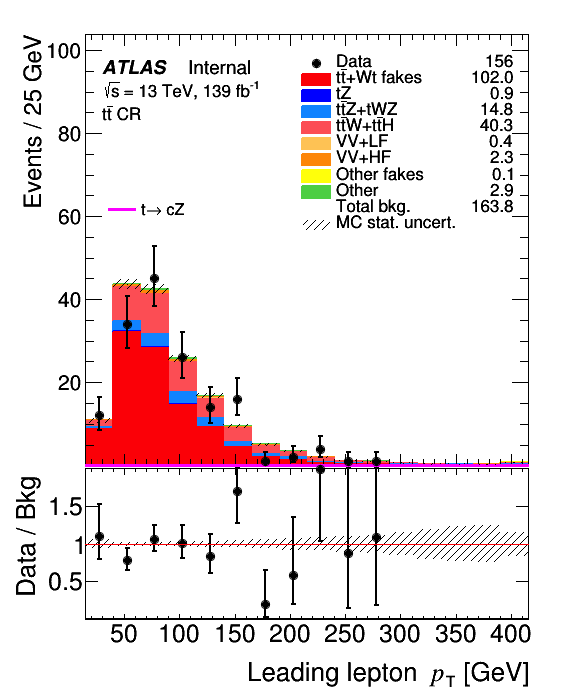
\includegraphics[width=.32\textwidth]{Chapters/CH6/figures/TTCR/lep1_pt} \\
		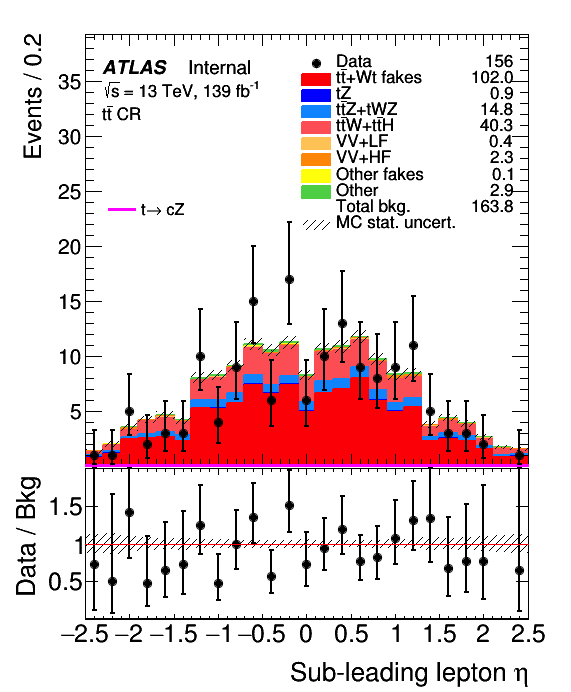
\includegraphics[width=.32\textwidth]{Chapters/CH6/figures/TTCR/lep2_eta} &
		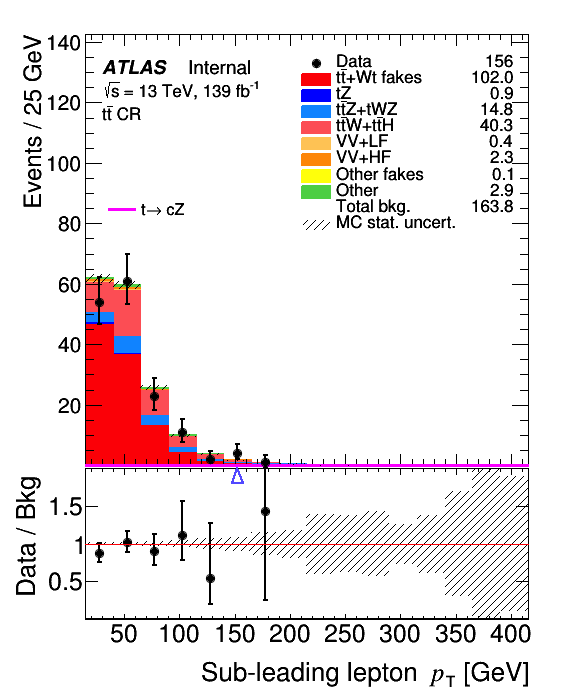
\includegraphics[width=.32\textwidth]{Chapters/CH6/figures/TTCR/lep2_pt} \\
		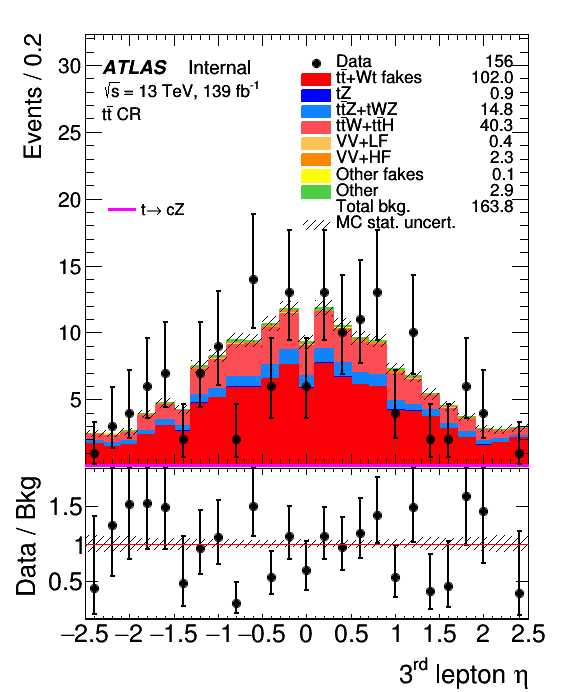
\includegraphics[width=.32\textwidth]{Chapters/CH6/figures/TTCR/lep3_eta} &
		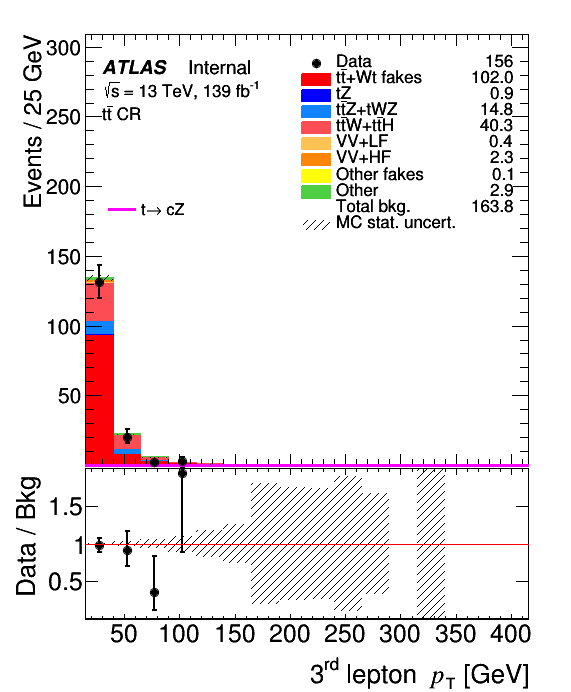
\includegraphics[width=.32\textwidth]{Chapters/CH6/figures/TTCR/lep3_pt} \\
	\end{tabular}
	\caption{Pre-fit distributions of kinematic variables of leptons for events selected in the \ttbar CR.
		\ErrStatOnly
	}%
	\label{fig:sel:cr:ttbar:leps}
\end{figure}

\begin{figure}[htbp]
	\centering
	\begin{tabular}{cc}
		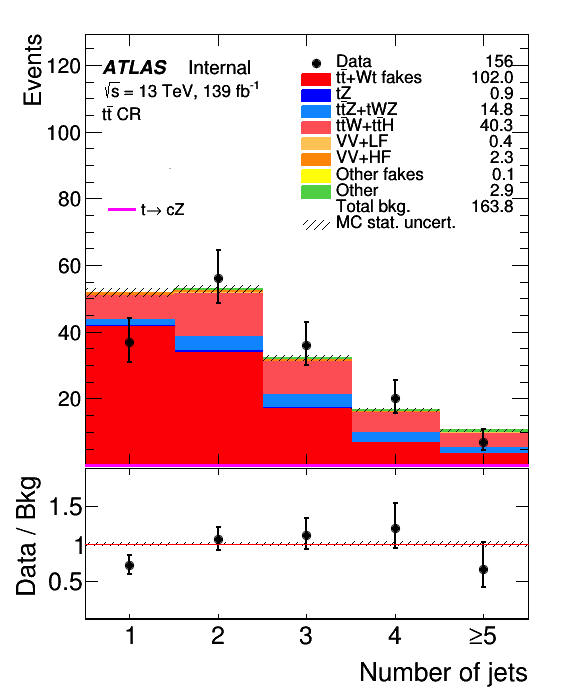
\includegraphics[width=.35\textwidth]{Chapters/CH6/figures/TTCR/nJets} &
		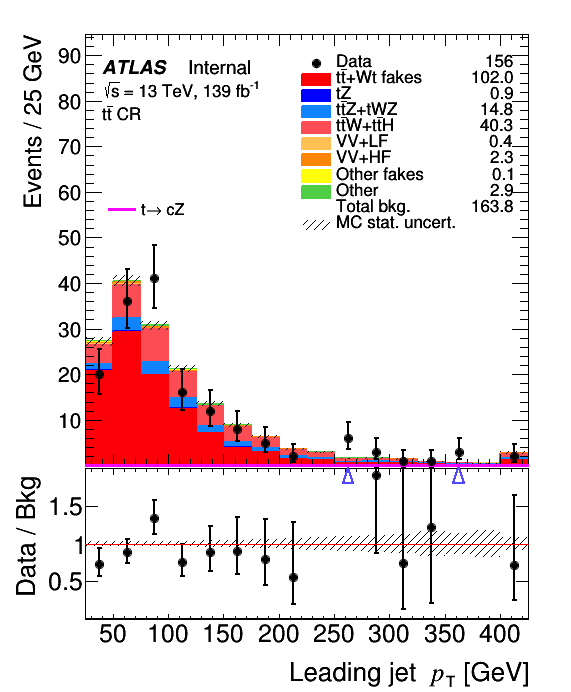
\includegraphics[width=.35\textwidth]{Chapters/CH6/figures/TTCR/jet_pt} \\
		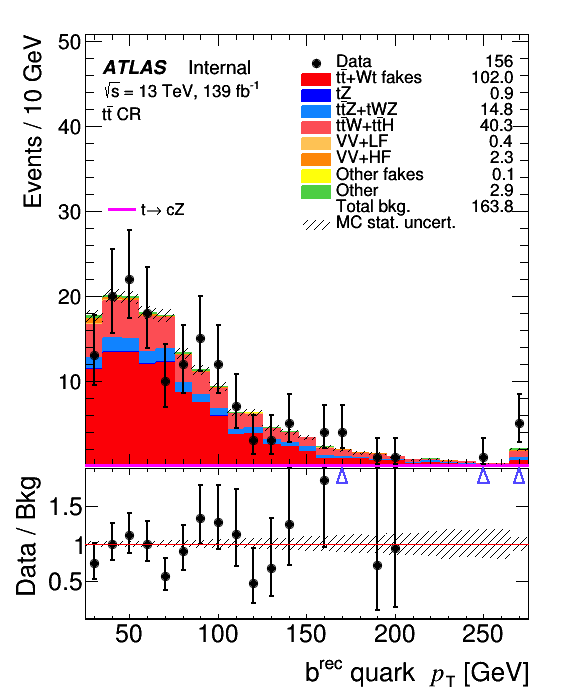
\includegraphics[width=.35\textwidth]{Chapters/CH6/figures/TTCR/b_pt} & 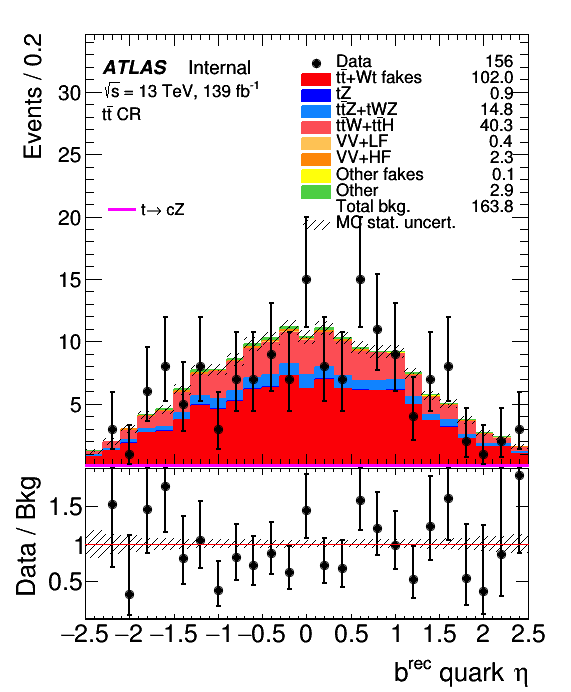
\includegraphics[width=.35\textwidth]{Chapters/CH6/figures/TTCR/b_eta} \\
	\end{tabular}
	\caption{Pre-fit distributions of kinematic variables of jets for events selected in the \ttbar CR.
		\ErrStatOnly
		\NoBDTGCut
		\Blinded
	}%
	\label{fig:sel:cr:ttbar:jets}
\end{figure}

\clearpage
\FloatBarrier
% -------------------------------------------------------------------------------
\subsubsection{\ttZ CR}
% -------------------------------------------------------------------------------
\Cref{fig:sel:cr:ttz:leps,fig:sel:cr:ttz:jets} show the distributions 
of kinematic variables for events selected in the \ttZ CR region.

\begin{figure}[!htbp]
	\centering
	\begin{tabular}{cc}
		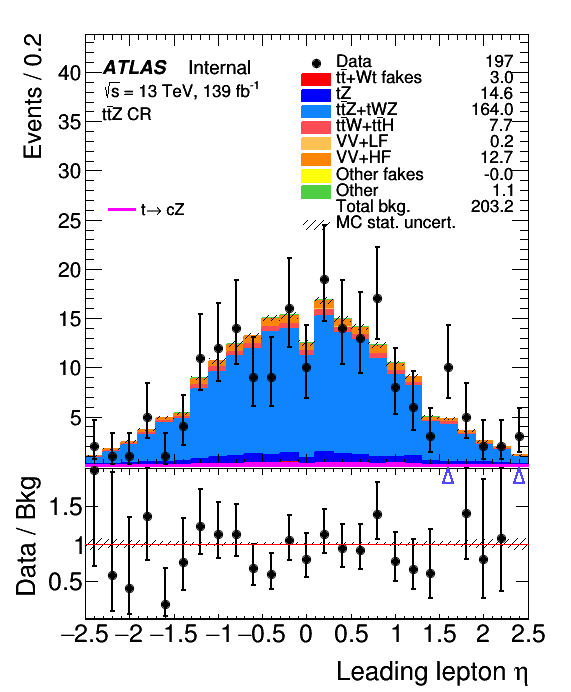
\includegraphics[width=.32\textwidth]{Chapters/CH6/figures/TTZCR/lep1_eta} &
		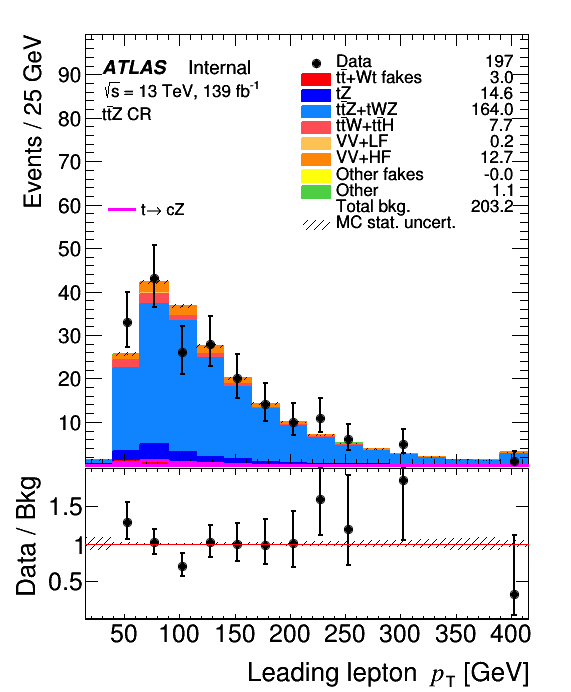
\includegraphics[width=.32\textwidth]{Chapters/CH6/figures/TTZCR/lep1_pt} \\
		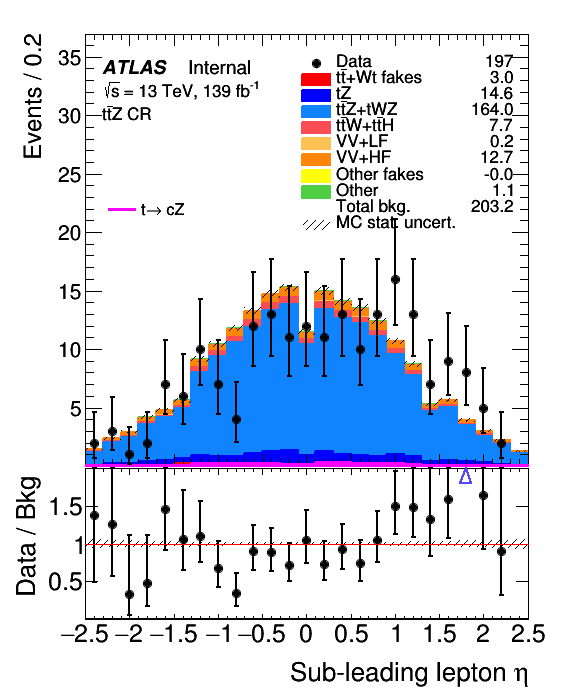
\includegraphics[width=.32\textwidth]{Chapters/CH6/figures/TTZCR/lep2_eta} &
		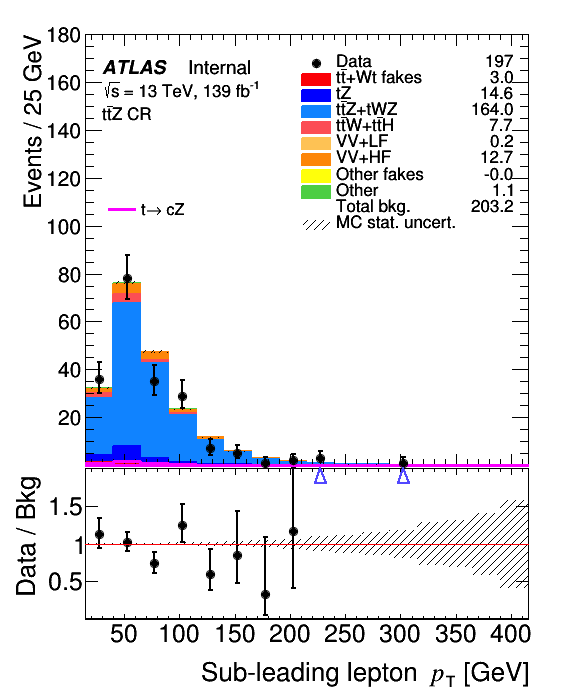
\includegraphics[width=.32\textwidth]{Chapters/CH6/figures/TTZCR/lep2_pt} \\
		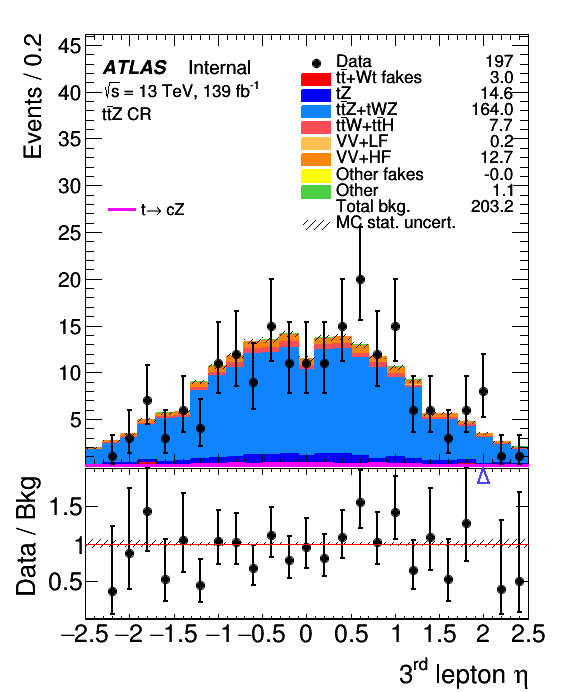
\includegraphics[width=.32\textwidth]{Chapters/CH6/figures/TTZCR/lep3_eta} &
		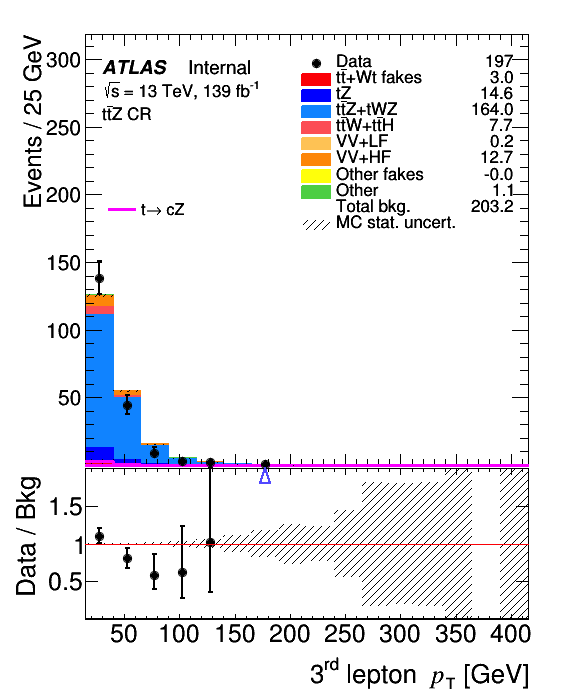
\includegraphics[width=.32\textwidth]{Chapters/CH6/figures/TTZCR/lep3_pt} \\
	\end{tabular}
	\caption{Pre-fit distributions of kinematic variables of leptons for events selected in the \ttZ CR.
		\ErrStatOnly
	}%
	\label{fig:sel:cr:ttz:leps}
\end{figure}

\begin{figure}[htbp]
	\centering
	\begin{tabular}{cc}
		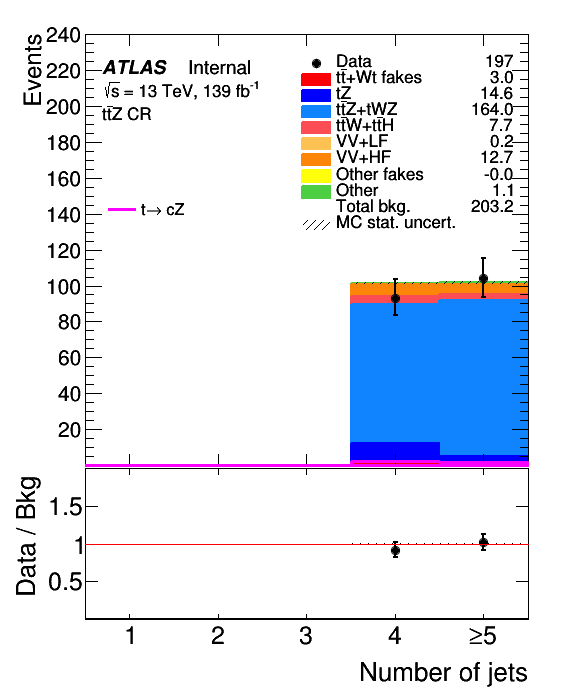
\includegraphics[width=.35\textwidth]{Chapters/CH6/figures/TTZCR/nJets} &
		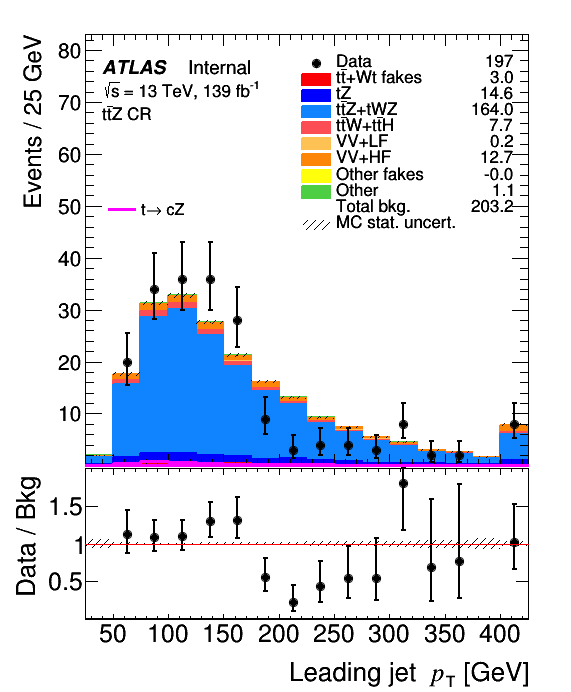
\includegraphics[width=.35\textwidth]{Chapters/CH6/figures/TTZCR/jet_pt} \\
		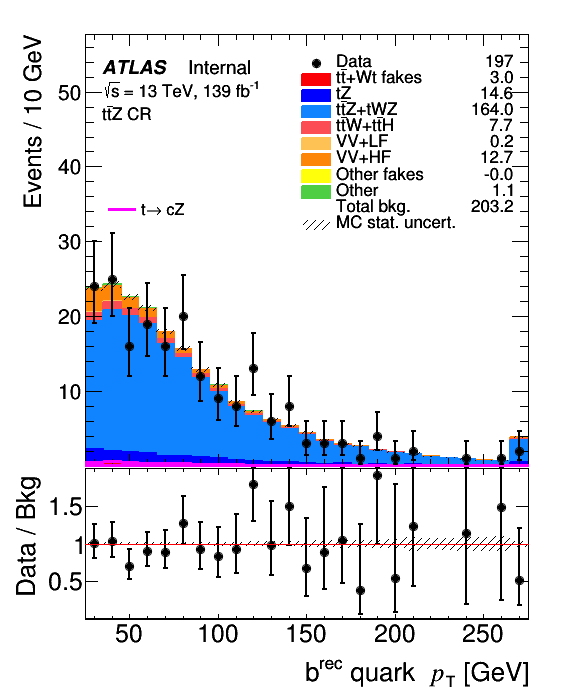
\includegraphics[width=.35\textwidth]{Chapters/CH6/figures/TTZCR/b_pt} &
		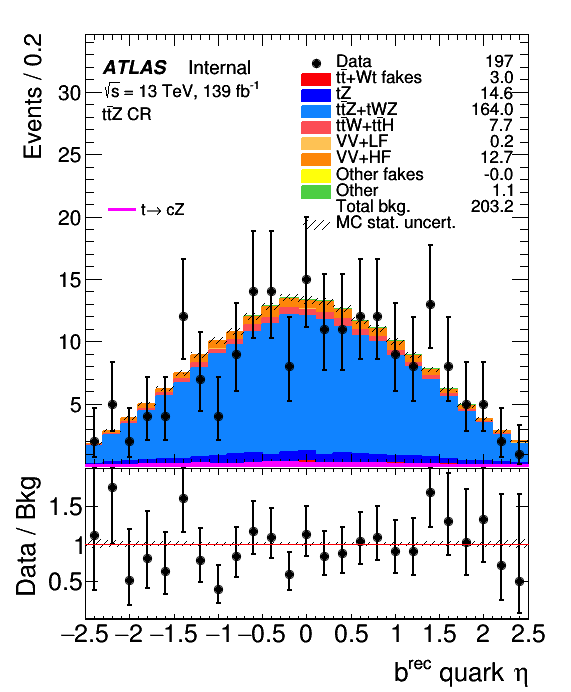
\includegraphics[width=.35\textwidth]{Chapters/CH6/figures/TTZCR/b_eta} \\
	\end{tabular}
	\caption{Pre-fit distributions of kinematic variables of jets for events selected in the \ttZ CR.
		\ErrStatOnly
		\NoBDTGCut
		\Blinded
	}%
	\label{fig:sel:cr:ttz:jets}
\end{figure}

\clearpage
\FloatBarrier
% -----------------------------------------------------------------------------
\subsubsection{Side-band CR1}
% -------------------------------------------------------------------------------
\Cref{fig:sel:cr:sb1tzc:leps,fig:sel:cr:sb1tzc:jets} show the distributions 
of kinematic variables for events selected in the side-band CR1 region. 

\begin{figure}[!htbp]
	\centering
	\begin{tabular}{cc}
		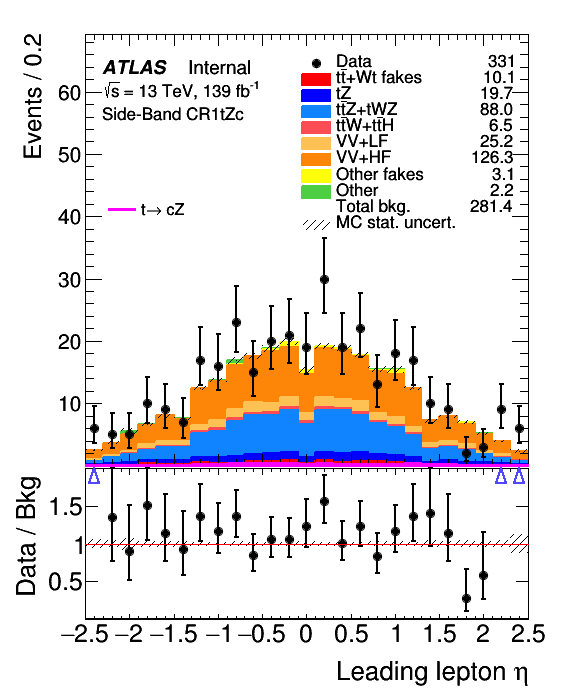
\includegraphics[width=.32\textwidth]{Chapters/CH6/figures/SBCR1/lep1_eta} &
		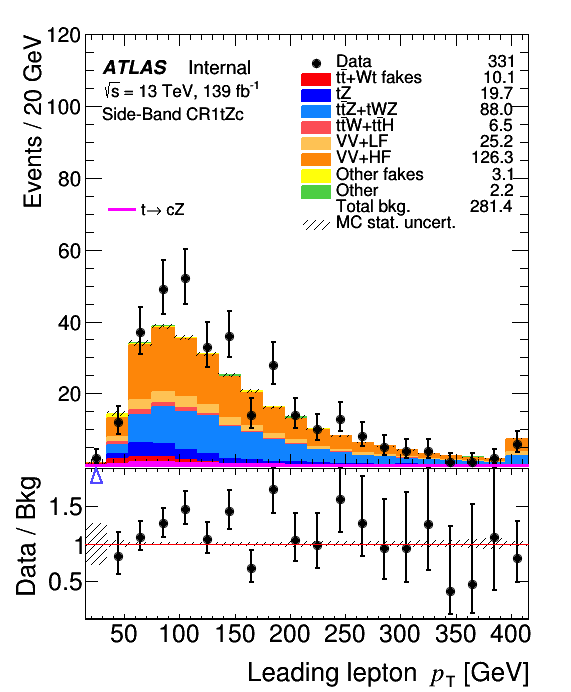
\includegraphics[width=.32\textwidth]{Chapters/CH6/figures/SBCR1/lep1_pt} \\
		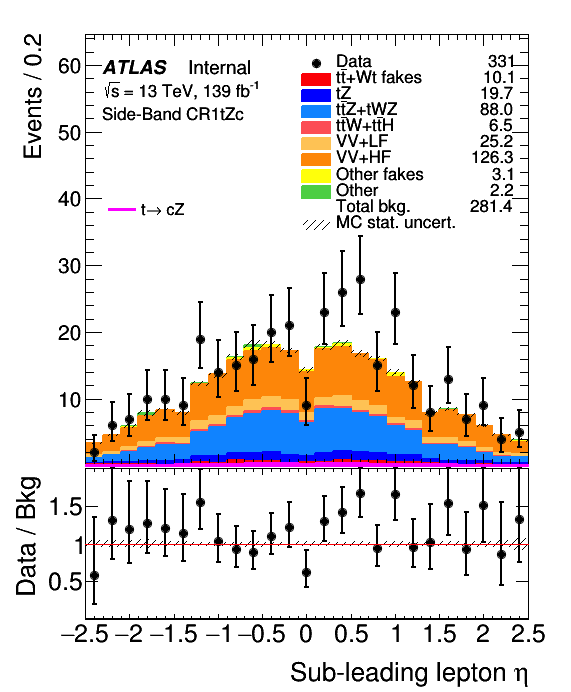
\includegraphics[width=.32\textwidth]{Chapters/CH6/figures/SBCR1/lep2_eta} &
		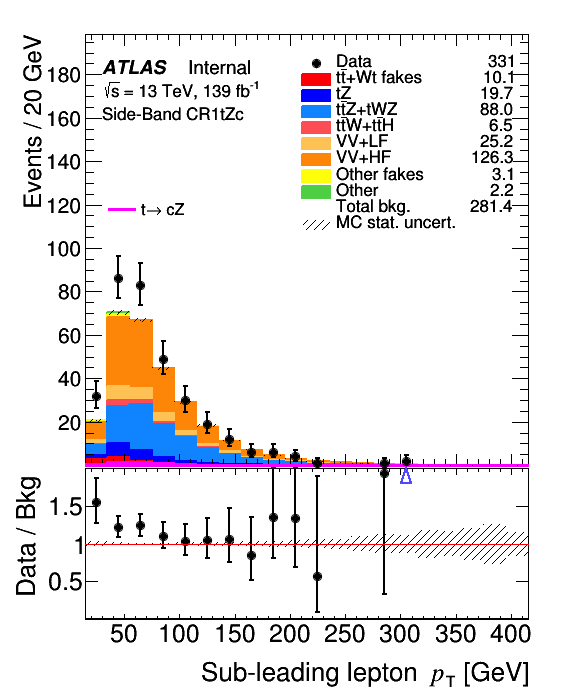
\includegraphics[width=.32\textwidth]{Chapters/CH6/figures/SBCR1/lep2_pt} \\
		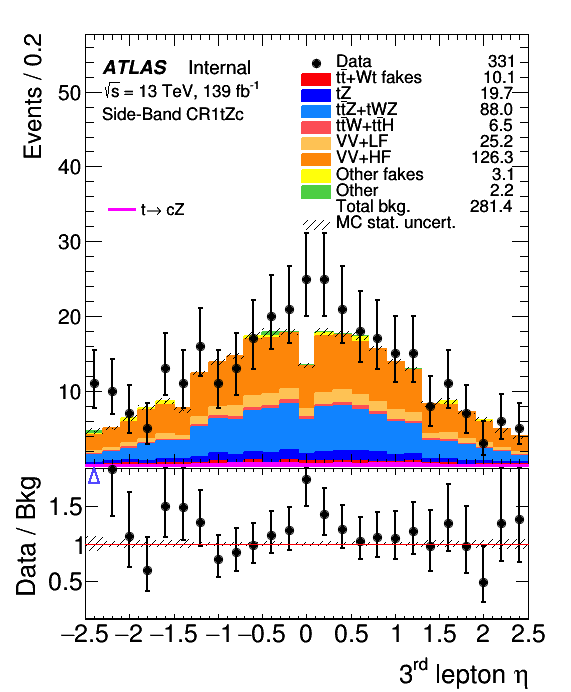
\includegraphics[width=.32\textwidth]{Chapters/CH6/figures/SBCR1/lep3_eta} &
		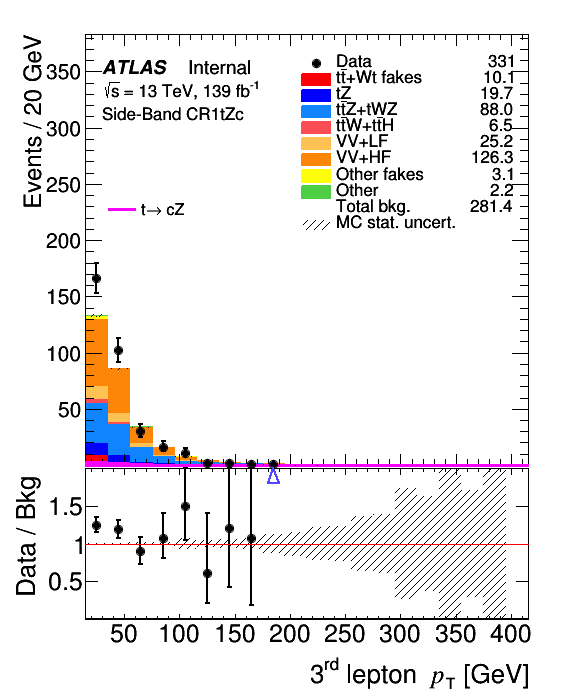
\includegraphics[width=.32\textwidth]{Chapters/CH6/figures/SBCR1/lep3_pt} \\
	\end{tabular}
	\caption{Pre-fit distributions of kinematic variables of leptons for events selected in the side-band CR1 region.
		\ErrStatOnly
	}%
	\label{fig:sel:cr:sb1tzc:leps}
\end{figure}

\begin{figure}[htbp]
	\centering
	\begin{tabular}{cc}
		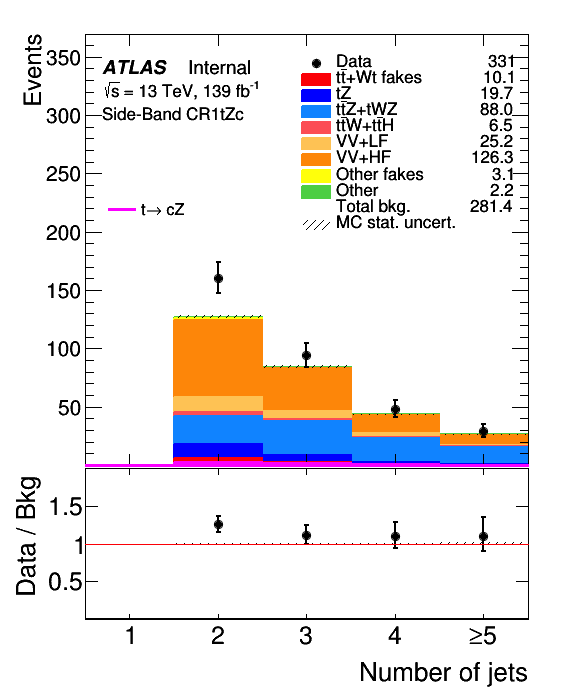
\includegraphics[width=.35\textwidth]{Chapters/CH6/figures/SBCR1/nJets}&
		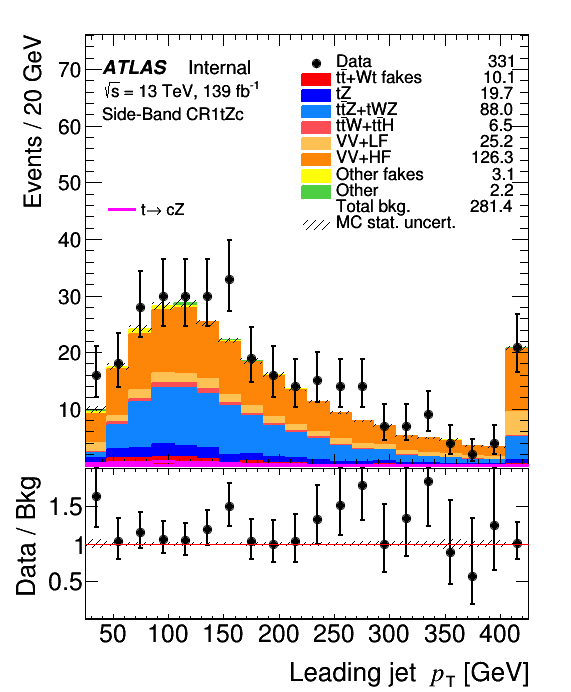
\includegraphics[width=.35\textwidth]{Chapters/CH6/figures/SBCR1/jet_pt} \\
		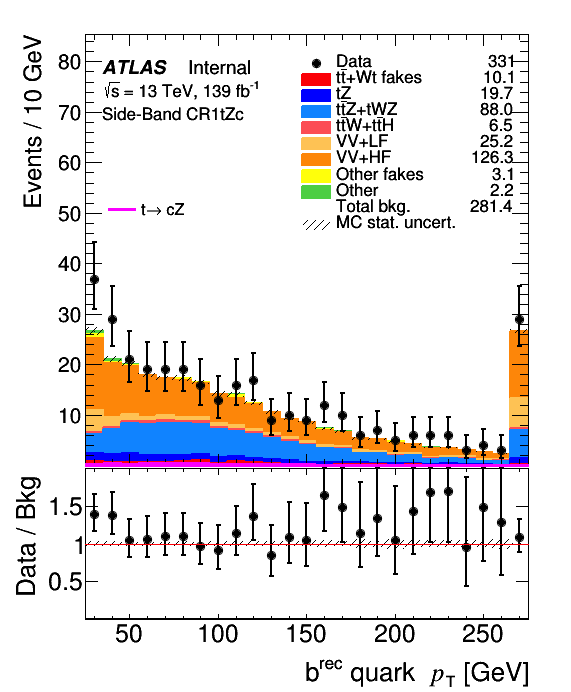
\includegraphics[width=.35\textwidth]{Chapters/CH6/figures/SBCR1/b_pt} &
		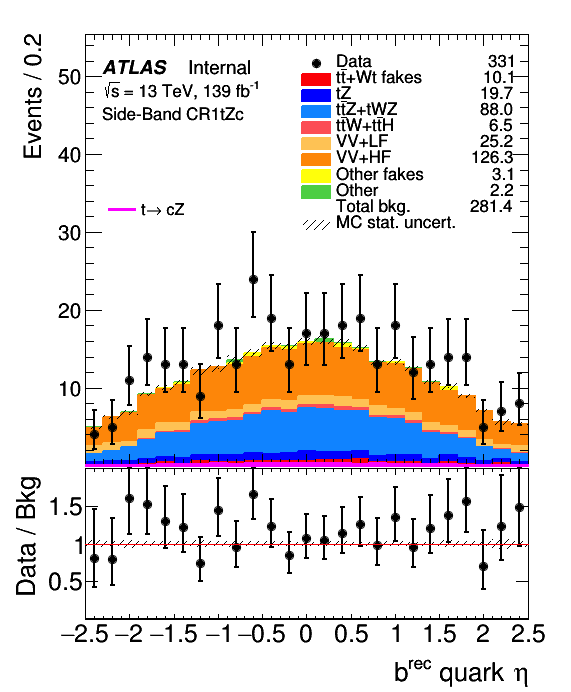
\includegraphics[width=.35\textwidth]{Chapters/CH6/figures/SBCR1/b_eta}\\
	\end{tabular}
	\caption{Pre-fit distributions of kinematic variables of jets for events selected in the side-band CR1 region.
		\ErrStatOnly
		\NoBDTGCut
		\Blinded
	}%
	\label{fig:sel:cr:sb1tzc:jets}
\end{figure}

\clearpage
\FloatBarrier
% -------------------------------------------------------------------------------
\subsubsection{Side-band CR2}
% -------------------------------------------------------------------------------
\Cref{fig:sel:cr:sb2:leps,fig:sel:cr:sb2:jets} show the distributions 
of kinematic variables for events selected in the side-band CR2 region.

\begin{figure}[!htbp]
	\centering
	\begin{tabular}{cc}
		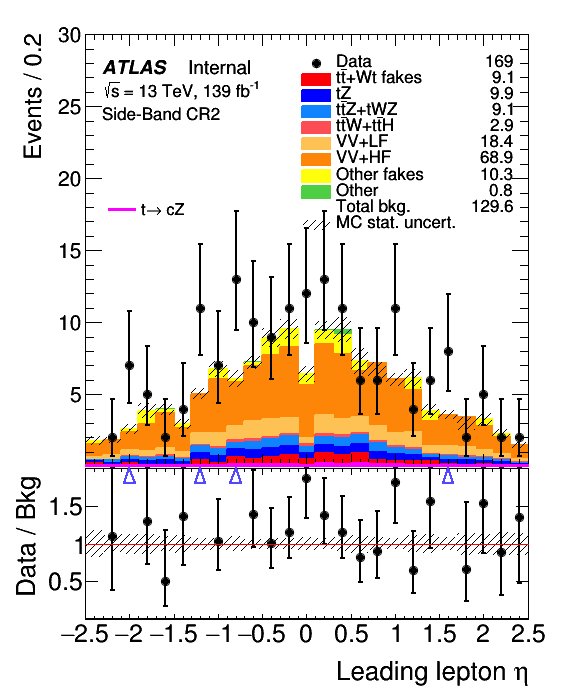
\includegraphics[width=.32\textwidth]{Chapters/CH6/figures/SBCR2/lep1_eta} &
		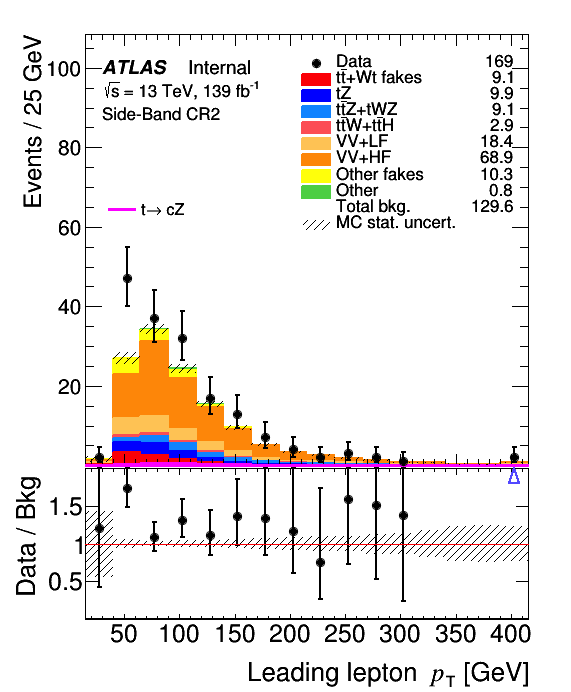
\includegraphics[width=.32\textwidth]{Chapters/CH6/figures/SBCR2/lep1_pt} \\
		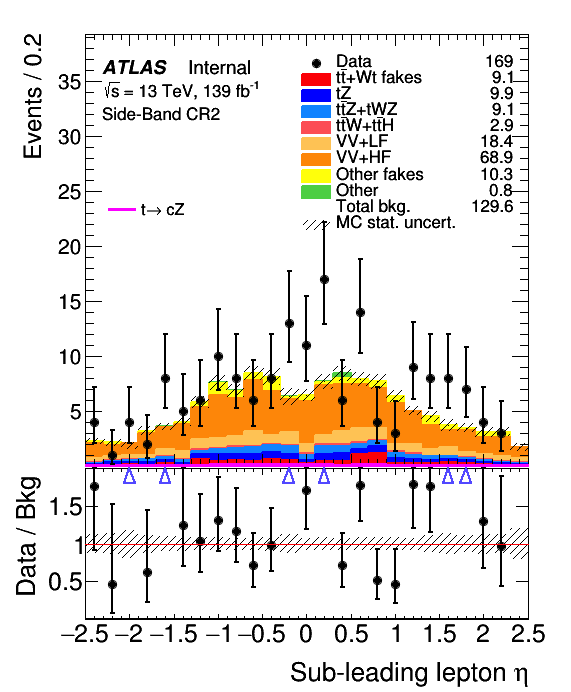
\includegraphics[width=.32\textwidth]{Chapters/CH6/figures/SBCR2/lep2_eta} &
		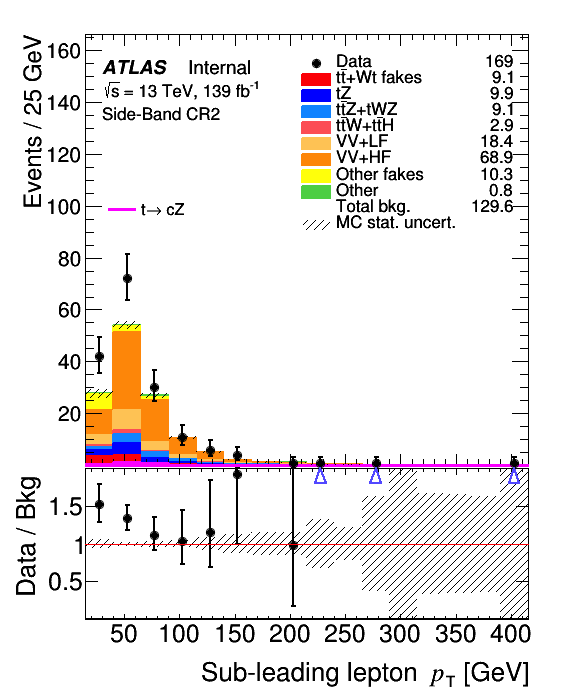
\includegraphics[width=.32\textwidth]{Chapters/CH6/figures/SBCR2/lep2_pt} \\
		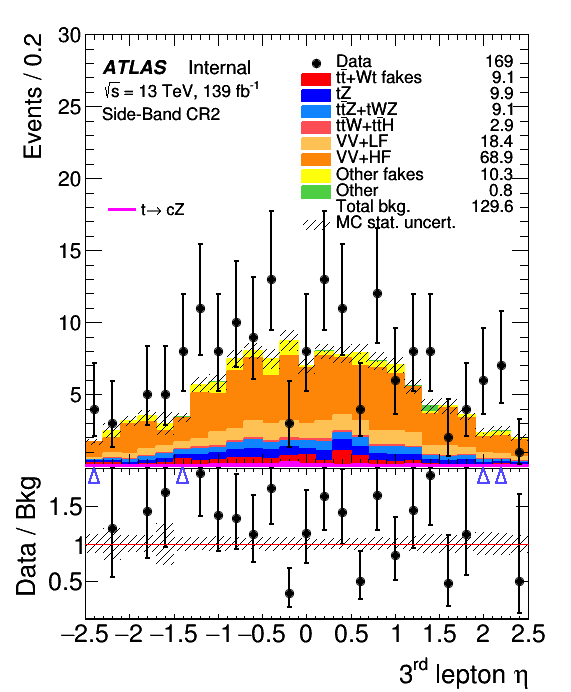
\includegraphics[width=.32\textwidth]{Chapters/CH6/figures/SBCR2/lep3_eta} &
		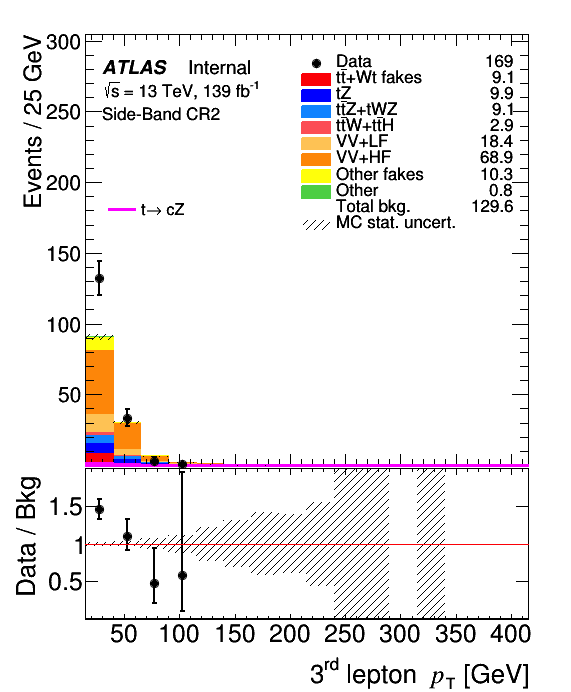
\includegraphics[width=.32\textwidth]{Chapters/CH6/figures/SBCR2/lep3_pt} \\
	\end{tabular}
	\caption{Pre-fit distributions of kinematic variables of leptons for events selected in the side-band CR2 region.
		\ErrStatOnly
	}%
	\label{fig:sel:cr:sb2:leps}
\end{figure}

\begin{figure}[htbp]
	\centering
	\begin{tabular}{cc}
		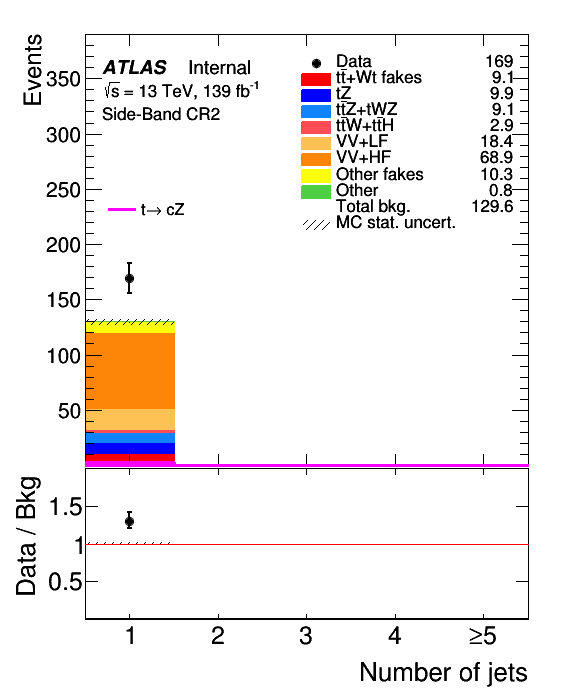
\includegraphics[width=.35\textwidth]{Chapters/CH6/figures/SBCR2/nJets} &
		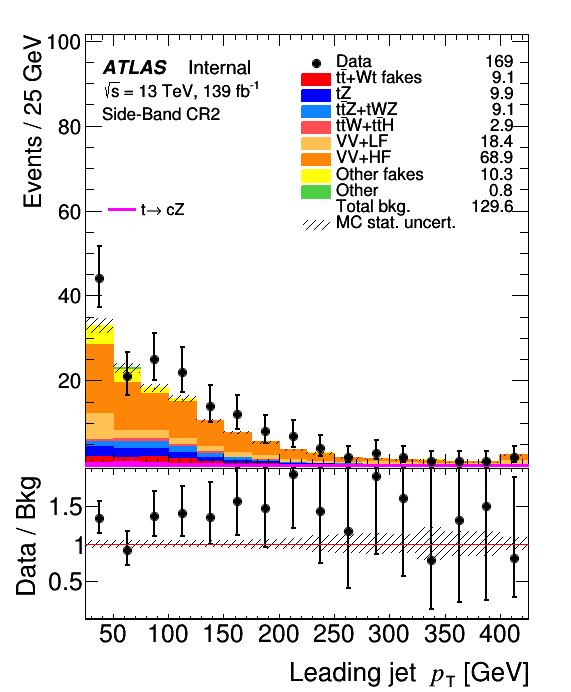
\includegraphics[width=.35\textwidth]{Chapters/CH6/figures/SBCR2/jet_pt} \\
		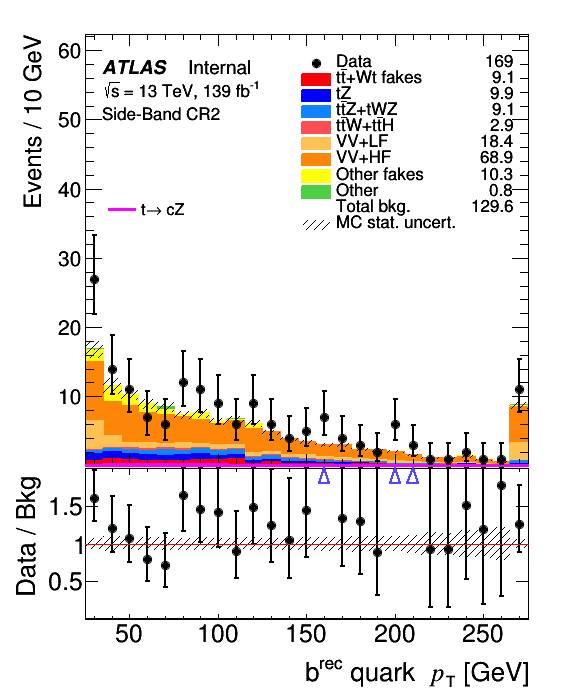
\includegraphics[width=.35\textwidth]{Chapters/CH6/figures/SBCR2/b_pt} &
		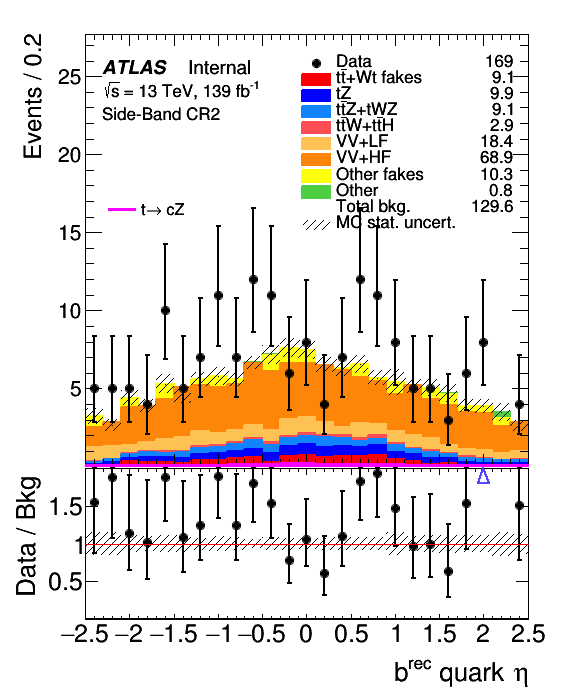
\includegraphics[width=.35\textwidth]{Chapters/CH6/figures/SBCR2/b_eta} \\
	\end{tabular}
	\caption{Pre-fit distributions of kinematic variables of jets for events selected in the side-band CR2 region.
		\ErrStatOnly
		\NoBDTGCut
		\Blinded
	}%
	\label{fig:sel:cr:sb2:jets}
\end{figure}


%\clearpage
%\subsection {Fake composition}
%The origin of the three leptons from \ttbar events was studied, to
%understand where the fake leptons come from and eventually define an
%uncertainty to take into account the different sources in the signal
%and control regions. The origin of the three leptons from \ttbar
%events is shown in \cref{fig:bkg:fakes:ttbar:comp}. As it can be
%seen, apart from the leptons for which the mother is the top quark
%(\SI{66}{\%} of the leptons in each event), the fake leptons come from
%either photon conversions (around \SI{5}{\%}, depending on the region)
%or from \Pqb-hadrons (around \SI{25}{\%}, depending on the region). \\
%Some differences can be noticed for the photon conversion and
%\Pqb-hadron fractions in the signal regions with respect to the \ttbar
%control region where the \ttbar background is controlled. To take into
%account this differences, a systematic uncertainties is added. 
%
%\begin{figure}[htbp]
%	\centering
%	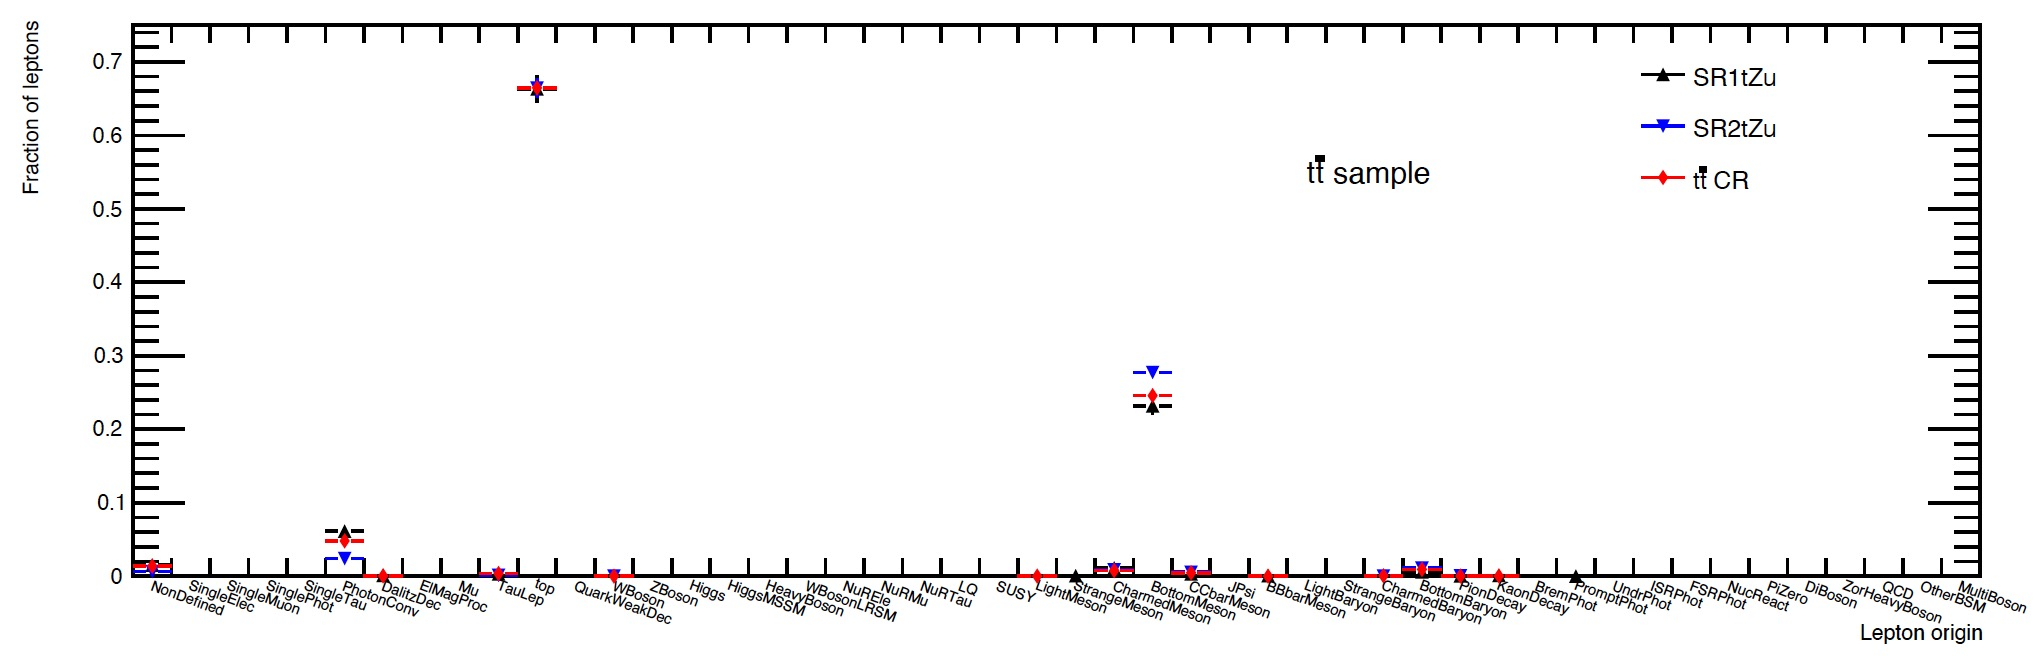
\includegraphics[width=1.\textwidth]{Chapters/CH5/figures/ttbar_leptons_origin}
%	\caption{Origin of the three leptons from \ttbar events in the
%		SR1\tZu, SR2\tZu and \ttbar CR. 
%	}%
%	\label{fig:bkg:fakes:ttbar:comp}
%\end{figure}
%
%\clearpage
%\FloatBarrier


\clearpage
\section{Separation of signal from background events}
\label{sec:separation}
\clearpage
\subsection {GBDT discriminant definition}
\clearpage
\subsection {Input variables}
\clearpage


